\documentclass{article}
\usepackage[T1]{fontenc}
\usepackage{lmodern}
\usepackage{graphicx}
\usepackage{amsmath,amssymb}
\usepackage[a4paper,margin=2cm]{geometry}
\usepackage[absolute,overlay]{textpos}
\setlength{\TPHorizModule}{1mm}
\setlength{\TPVertModule}{1mm}
\usepackage[indonesian]{babel}
\usepackage{hyperref}
\setlength{\emergencystretch}{2em}
% unit: Halaman 6

\begin{document}

% === Halaman 6 (llm) ===

\begin{itemize}
    \item \textbf{Case 1}: Bagaimana Alice memastikan pesan-pesannya tidak dapat dibaca oleh penyadap (\textit{eavesdropper}) yang menguping komunikasinya dengan Bob?
\end{itemize}

\vspace{40mm}

$\rightarrow$ masalah kerahasiaan pesan (\textit{confidentiality})

% deskripsi: Diagram ilustrasi komunikasi antara Alice dan Bob yang disadap oleh Eve (eavesdropper), menunjukkan aliran pesan dari Alice ke Bob dengan panah yang bercabang menuju Eve.
% bbox normalisasi: [0.2200, 0.3300, 0.7300, 0.7200]
\begin{textblock*}{107.10mm}(46.20mm,98.01mm)
\noindent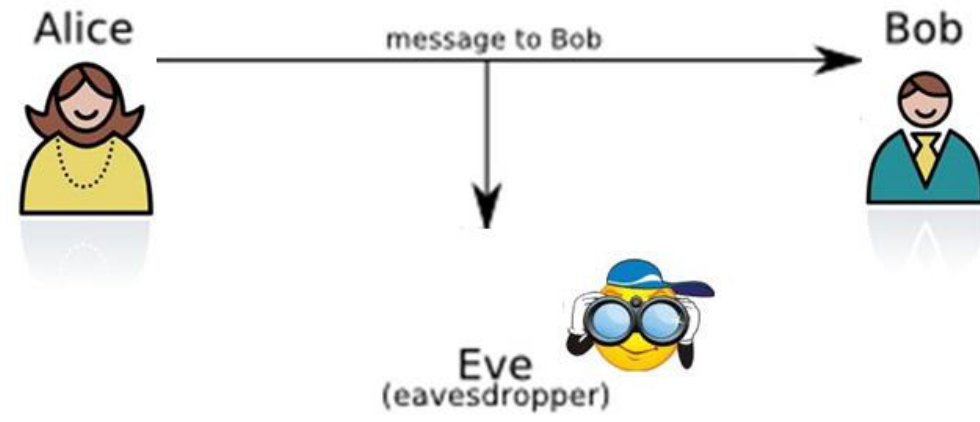
\includegraphics[width=107.10mm,height=115.83mm]{../../images/llm/page_006_img_01.png}%
\end{textblock*}

\end{document}
